%%
%% ****** ljmsamp.tex 13.06.2018 ******
%%
\documentclass[
11pt,%
tightenlines,%
twoside,%
onecolumn,%
nofloats,%
nobibnotes,%
nofootinbib,%
superscriptaddress,%
noshowpacs,%
centertags]%
{revtex4}
\usepackage{ljm}

\usepackage{makecell}

\begin{document}

\titlerunning{Parallel global search algorithm with local tuning} % for running heads
%\authorrunning{First-Author at al.} % for running heads
\authorrunning{Barkalov, Gergel, Lebedev} % for running heads

\title{Parallel Global Search Algorithm with Local Tuning\\ 
for Solving Mixed-Integer Global Optimization Problems}
% Splitting into lines is performed by the command \\
% The title is written in accordance with the rules of capitalization.

\author{\firstname{K.~A.}~\surname{Barkalov}}
\email[E-mail: ]{konstantin.barkalov@itmm.unn.ru}
\affiliation{Lobachevsky State University of Nizhni Novgorod, Gagarin ave. 23, Nizhni Novgorod, 603950 Russia}

\author{\firstname{V.~P.}~\surname{Gergel}}
\email[E-mail: ]{gergel@unn.ru}
\affiliation{Lobachevsky State University of Nizhni Novgorod, Gagarin ave. 23, Nizhni Novgorod, 603950 Russia}

\author{\firstname{I.~G.}~\surname{Lebedev}}
\email[E-mail: ]{ilya.lebedev@itmm.unn.ru}
\affiliation{Lobachevsky State University of Nizhni Novgorod, Gagarin ave. 23, Nizhni Novgorod, 603950 Russia}
%\noaffiliation % If the author does not specify a place of work.

\firstcollaboration{(Submitted by V.~V.~Voevodin)} % Add if you know submitter.
%\lastcollaboration{ }

\received{February 20, 2021} % The date of receipt to the editor, i.e. December 06, 2017


\begin{abstract} % You shouldn't use formulas and citations in the abstract.
In this paper, we consider mixed-integer global optimization problems and propose a parallel algorithm for solving problems of this class based on information-statistical approach for solving continuous global optimization problems. Within this algorithm, we suggest using a local tuning scheme based on the assumption that the multiextremality of the discussed problem is weak. 
We also compare the sequential version of the algorithm with other similar methods.
The effectiveness of parallelizing the algorithm has been confirmed by solving a series of mixed-integer global optimization problems on the Lobachevsky supercomputer.
\end{abstract}

\subclass{90C26, 90C30} % Enter 2010 Mathematics Subject Classification.

\keywords{Global optimization, Non-convex constraints, Mixed-integer problems, Local tuning, Parallel algorithms} % Include keywords separeted by comma.

\maketitle

% Text of article starts here.

\section{Introduction}

Our research focuses on global optimization problems and parallel methods for their solution. Solving problems of this class requires substantial computational power since the global optimum as an integral characteristic of the problem requires the investigation of the entire search domain. Thus, the search for the global optimum is reduced to the construction of some coverage (as a rule, uneven) in the range of parameter change. This draws a particular interest to mixed-integer global optimization problems since it is more difficult to construct estimates of the optimum for such problems as compared to the continuous integer problems. 

So, it is quite typical when some of the parameters in the applied optimization problems are discrete. In this case, discrete parameters have, as a rule, a small number of values and can determine, for example, the grade of the material used, or the variation of the standard arrangement of parts, etc.
At the same time, the objective function and constraints are usually specified not explicitly, but in the form of some algorithm for calculating their values at the points of the search domain, i.e. they represent black-box functions. The process of checking the constraints and calculating the value of the objective function at a certain point (hereinafter referred to as trial) requires numerical simulation and is a time-consuming operation. 

An extensive literature is devoted to methods for solving mixed-integer problems (see, for example, reviews \cite{Burer,Boukouvala}). Known deterministic methods for solving problems of this class are based, as a rule, on the Branch-and-Bound \cite{Belotti} or Branch-and-Reduce approach \cite{Vigerske}. Such problems may also be solved by nature-inspired algorithms \cite{Deep,Schluter}, which in one way or another are based on a random search.

Let us highlight the key points that are specific to the construction of parallel algorithms for solving mixed-integer global optimization problems. There are several ways to parallelize the search process.
First, we can parallelize one trial, i.e. calculate functions of a problem at one point in the search domain. This approach will accelerate the calculations, but on the other hand, will have to be tailored for each particular problem.
Second, we can parallelize the implementation of the computational rules of the algorithm that ensure the selection of a point for the next trial. In this case, the method of parallelization will depend on the specific class of algorithm. However, these rules are often quite simple, which makes their parallelization impractical.
Third, it is possible to organize parallel execution of several trials during one search iteration. We will use this approach in this work due to its efficiency (it provides parallelization of the exact part of the computational process responsible for the bulk of the calculations) and generality (applicable to a wide class of global optimization algorithms).

In this paper, we propose a new parallel method for solving mixed-integer problems based on an information-statistical approach to solving global optimization problems \cite{Strongin2000,Strongin2013}. 

Within this approach: 
\begin{itemize}
	\item 
	solving multidimensional problems is reduced to solving equivalent one-dimensional problems, the corresponding reduction is based on the use of space-filling curves;
	\item 
	when solving constrained optimization problems, each constraint is taken into account and processed separately, and penalty functions are not used;
	\item
	taking into account the information on the inhomogeneous behavior of the problem functions in different subdomains of the search domain makes it possible to speed up the process of finding a solution by combining the procedures for local refinement of the current best solution and its global update;
	\item 
	parallelization of the search process is carried out by simultaneous calculation of several values of the objective function at different points of the search domain during each iteration.	
\end{itemize}

To provide a proper representation of the results of the study, we structured the text of the article as follows.
Section 2 provides a brief description of the dimension reduction scheme using space-filling curves, as well as an index scheme for considering constraints. It also contains the formulation of a parallel index algorithm for solving continuous global optimization problems.
Section 3 outlines a way to take into account the local properties of the problem functions to speed up the convergence of the algorithm.
Section 4 proposes an approach to generalize the parallel index algorithm to solve mixed-integer problems. This method allows reducing the solution of the mixed-integer problem to the solution of an information-related set of continuous optimization problems which can be performed in parallel.
Section 5 contains the results of numerical experiments. There we compare the sequential version of the algorithm with known alternatives and also demonstrate the efficiency of parallelizing the algorithm with local tuning when solving the multiextremal mixed-integer problem series on a supercomputer. 
Section 6 concludes the paper.

\section{Parallel global optimization algorithm\protect\\
and dimensionality reduction}

Let us consider a global optimization problem with continuous parameters of the form
\begin{eqnarray}\label{problem}
&\varphi(y^\ast)=\min{\left\{\varphi(y):y\in D, \; g_i(y)\leq 0, \; 1 \leq i \leq m\right\}},\\
&D=\left\{y\in R^N: a_j\leq y_j \leq b_j, 1\leq j \leq N \right\}.\label{D}
\end{eqnarray}
We will assume that objective function $\varphi(y)$ (hereafter denoted by $g_{m+1}(y)$) and the left-hand sides $g_i(y), \; 1\leq i \leq m,$ of the constraints satisfy the Lipschitz condition 
\[
\left|g_i(y_1)-g_i(y_2)\right|\leq L_i\left\|y_1-y_2\right\|, \;1\leq i\leq m+1, \; y_1,y_2 \in D,\;
\]
with a priori unknown constants $L_i, \; 1 \leq i \leq m+1$. 

The assumption that the Lipschitz condition is satisfied is typical for many approaches to the construction of parallel algorithms for global optimization \cite{Evtushenko2009,Zilinskas2011}. In this case, the solution of a multidimensional optimization problem requires algorithms to be adjusted for solving one-dimensional problems, see, for example, methods based on partitions of the search domain \cite{Zilinskas2014,Sergeyev2017}.

In this work, we will use an approach to reducing multidimensional problems to one-dimensional problems based on space-filling curves.
Using mappings of the Peano-Hilbert curve $y(x)$ type, which project the segment $[0,1]$ onto the $N$-dimensional domain (\ref{D}),
we can reduce the multidimensional conditional minimization problem in the domain $D$ to a one-dimensional conditional minimization problem in the segment $[0,1]$
\begin{equation}\label{problem1}
\varphi(y(x^\ast))=\min \left\{\varphi(y(x)): x \in [0,1], \; g_i(y(x))\leq 0, \; 1 \leq i \leq m\right\}.
\end{equation}

Methods for constructing numerical approximations of Peano-Hilbert curves $y(x)$ (called \textit{evolvents}) are discussed in \cite{Sergeyev2013}. These evolvents are fractals generated by an iterative process. They fill in the hypercube $D$ with accuracy $2^{-M}$, where integer $M>0$ is the evolvent construction parameter. 
Examples of evolvents with different values of $M$  for the dimensionality $N=3$ are shown in Fig.~\ref{evolvents}.

\begin{figure}[ht]
\begin{minipage}{0.4\linewidth}
\center{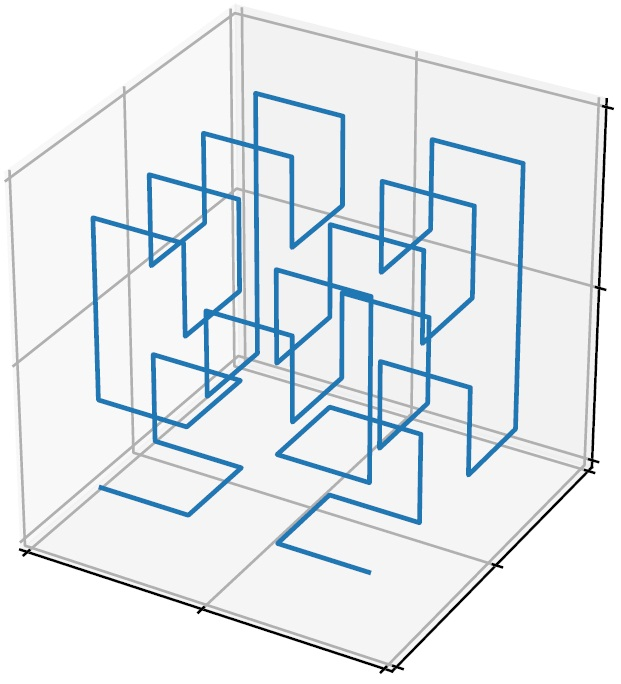
\includegraphics[width=1.0\linewidth]{fig1b.JPG} \\ (a)}
\end{minipage}
\begin{minipage}{0.4\linewidth}
\center{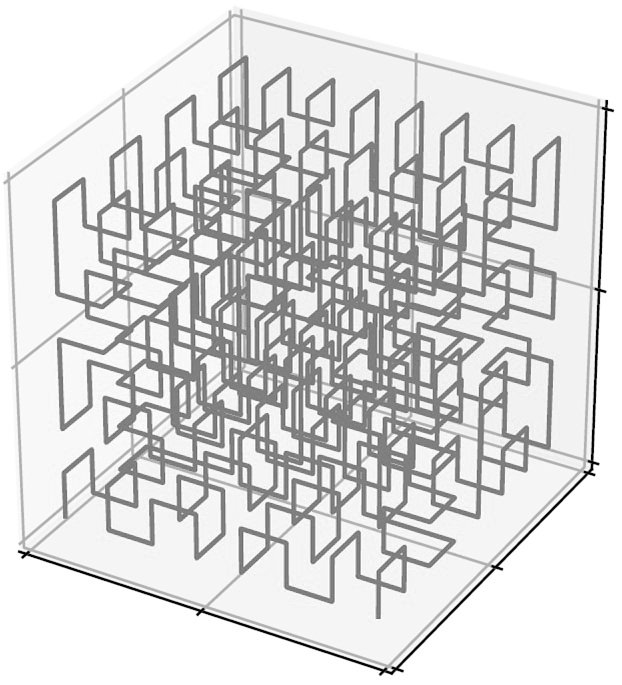
\includegraphics[width=1.0\linewidth]{fig1c.JPG} \\ (b)}
\end{minipage}
\caption{Evolvents in three dimensions with (a) $M=3$ and (b) $M=4$}
\label{evolvents}
\end{figure}

We shall consider the problem (\ref{problem1}) under the assumption that the functions $g_i(y(x))$ are defined and computable only on the corresponding sets
\[
Q_1=[0,1], \; Q_{i+1}=\left\{x \in Q_i : g_i(y(x)) \leq 0 \right\}, \; 1 \leq i \leq m.
\]

These conditions allow for the classification of points $x \in [0,1]$ in accordance with the number of constraints $\nu(x)$  calculated at this point. The \textit{index} $\nu(x)$ can also be determined using conditions

\begin{equation}\label{nu}
g_i(y(x)) \leq 0, \; 1 \leq i < \nu, \; g_\nu(y(x))>0,
\end{equation}
where the last inequality is excluded from consideration if  $\nu=m+1$.

The indicated dimensionality reduction scheme associates a multidimensional problem with a Lipschitz objective function and Lipschitz constraints with a one-dimensional problem in which the corresponding functions satisfy the uniform  H{\"o}lder condition (see \cite{Sergeyev2013}), i.e.,
\[
\left|g_i(y(x_1))-g_i (y(x_2))\right| \leq H_i \left|x_1-x_2 \right|^{1/N}, \; x_1,x_2\in [0,1], \; 1\leq i \leq m+1,
\]
where $N$ is the dimensionality of the original multidimensional problem, and H{\"o}lder coefficients $H_i$ are related to Lipschitz constants $L_i$ of the original problem by the relation  $H_i \leq 2L_i \sqrt{N+3}$.

Thus, \textit{a trial} at a point $x^k \in [0,1]$ performed during the $k$-th iteration of the algorithm will feature the following steps:
\begin{itemize}
	\item determine \textit{image} $y^k=y(x^k)$ in accordance with the mapping $y(x)$;
	\item calculate values $g_1(y^k),..., g_\nu(y^k),$ where $\nu = \nu(x^k)$ is from (\ref{nu}). 
\end{itemize}
A value pair
\begin{equation} \label{trial_result}
 \{ \nu=\nu(x^k), \; z^k=g_\nu(y(x^k)) \} 
\end{equation}
generated by the trial at a point $x^k \in [0,1]$, will be referred to as \textit{trial outcome}.

Let us consider a parallel algorithm for solving constrained global optimization problems proposed in  \cite{Strongin2000,Strongin2013} and based on an index scheme for the accounting of constraints.
To describe a parallel algorithm, we will assume that we have $p$ computational elements (nodes, processors, or cores) at our disposal, which will be used for parallel execution of $p$ trials simultaneously. 

During the first iteration of the method, $p$ trials trials are carried out in parallel at different arbitrary points $x^i\in(0,1)$, $1\leq i \leq p$.
Let $n\geq 1$ iterations of the method be performed with trials at $k=np$ points $x^i, 1\leq i \leq k$. Then points $x^{k+1},...,x^{k+p}$ of the search trials during the $(n+1)$-th iteration are determined according to the following rules.

\begin{enumerate}
\item 
Renumber the points $x^1,...,x^k$ of the previous trials with subscripts in ascending order of coordinate values
\begin{equation}\label{Eq:17}
0=x_0<x_1<...<x_i<...<x_k<x_{k+1}=1,
\end{equation}
and assign $z_i=g_\nu(y(x_i))$, $\nu=\nu(x_i)$, $1 \leq i \leq k$; points $x_0=0$ and $x_{k+1}=1$ are introduced additionally, values $z_0$ and $z_{k+1}$ are not set.
\item
Classify indexes  $i,1\leq i \leq k$, of the trial points from  (\ref{Eq:17}) by the number of constraints that are met at these points by constructing the sets
\begin{equation}\label{Eq:18}
I_\nu = \left\{i: 1 \leq i \leq k,\ \nu = \nu(x_i)\right\},\ 1 \leq \nu \leq m+1,
\end{equation}
containing the indices of all points $x_i,1\leq i \leq k$, with indices equal to the same value $\nu$. The boundary points $x_0=0$ and $x_{k+1}=1$ are interpreted as having zero indices, and an additional set $I_0=\{0,k+1\}$ is assigned to them. 

Determine the maximum value of indices
\begin{equation}\label{Eq:19}
V=\max \left\{\nu = \nu(x_i), \ 1\leq i \leq k\right\}.
\end{equation}
\item
For all values of $\nu, \ 1\leq \nu \leq m+1$, calculate the values  
\begin{equation}\label{Eq:20}
\mu_\nu = \max \left\{ \frac{\left|z_i-z_j\right|}{\left(x_i-x_j\right)^{1/N}} : i,j \in I_\nu, j<i\right\}.
\end{equation}
If set $I_\nu$ contains less than two elements or if $\mu_\nu$ from (\ref{Eq:20}) is equal to zero, then use the value $\mu_\nu=1$.
\item
For all non-empty sets $I_\nu$, $1 \leq \nu \leq m+1$, calculate values
\begin{equation}\label{Eq:21}
  z^\ast_\nu =  
   \begin{cases}
    -\epsilon_\nu,  \nu < V, \\
    \min{\left\{g_\nu(x_i):i\in I_\nu\right\}}, \nu = V,
   \end{cases}
\end{equation}
where $V$ is the maximum index value and the vector
\begin{equation}\label{Eq:22}
\epsilon _R=\left(\epsilon_1,...,\epsilon_m\right),
\end{equation}
with positive components (also referred to as \textit{reserve vector}) is the algorithm parameter.
\item
For each interval $(x_{i-1},x_i)$,$1 \leq i \leq k+1$, calculate the \textit{characteristics} $R(i)$: 
\begin{eqnarray}\label{R}
&R(i)=\Delta_i+ \frac{(z_i-z_{i-1})^2}{(r_\nu\mu_\nu)^2\Delta_i}-2\frac{z_i+z_{i-1}-2z^\ast_\nu}{r_\nu\mu_\nu},\;\; \nu=\nu(x_{i-1})=\nu(x_i),\nonumber \\
&R(i)= 2\Delta_i-4\frac{z_i-z^\ast_\nu}{r_\nu\mu_\nu},\;\; \nu(x_{i-1})<\nu(x_i)=\nu,\\
&R(i)= 2\Delta_i-4\frac{z_{i-1}-z^\ast_\nu}{r_\nu\mu_\nu},\;\; \nu = \nu(x_{i-1})>\nu(x_i),\nonumber
\end{eqnarray}
where $\Delta_i=(x_i-x_{i-1})^{1/N}$, and values $r_\nu>1, 1\leq\nu\leq m+1$, are the algorithm parameters.
\item
Sort characteristics $R(i)$, $1\leq i \leq k+1$, in descending order 	
\begin{equation}\label{Eq:23}
R(t_1)\geq R(t_2)\geq ... \geq R(t_{k})\geq R(t_{k+1})
\end{equation}
and select $p$ intervals with numbers $t_j, 1\leq j \leq p,$ corresponding to the largest characteristics.
\item
Conduct $p$ new trials in parallel at points $x^{k+j}, 1 \leq j \leq p$, calculated by the formulas
\begin{gather*}
x^{k+j}=\frac{x_{t_j}+x_{t_j-1}}{2}, \; \nu(x_{t_j-1})\neq \nu(x_{t_j}), \\
x^{k+j}=\frac{x_{t_j}+x_{t_j-1}}{2}- \frac{\mathrm{sign}(z_{t_j}-z_{t_j-1})}{2r_\nu}\left[\frac{\left|z_{t_j}-z_{t_j-1}\right|}{\mu_\nu}\right]^N, \; \nu(x_{t_j-1})=\nu(x_{t_j})=\nu. \\
\end{gather*} 

\end{enumerate}

The algorithm stops if the condition $\Delta_{t_j}\leq \epsilon$ is satisfied at least for one of the numbers $t_j, 1\leq j \leq p$; here $\epsilon>0$ is the target accuracy of the solution.

This way of organizing parallel computing has the following rationale. The characteristics of intervals (\ref{R}) used in the computational rules of the algorithm can be considered as some estimates of the probability of detecting a global minimum point in these intervals. Inequalities (\ref{Eq:23}) order the intervals according to their characteristics, and trials are carried out in parallel in the first $p$ intervals with the highest probabilities.

A detailed description of the algorithm convergence theory is presented in \cite{Strongin2000,Strongin2013}.
The role of the algorithm parameters ($r_\nu>1$ and $\epsilon_\nu>0, 1\leq\nu\leq m+1$) is discussed in \cite{Strongin2020}.
The described algorithm can also be used to solve multicriteria optimization problems \cite{Gergel2020}.

\section{Local tuning for global optimization algorithm}

One of the important properties of the problems under consideration is that, in many cases, the behavior of functions in the multiextremal optimization problem is inhomogeneous in different search subdomains. In some subdomains, the values of functions can change quite quickly, which will correspond to large values of the Lipschitz constant in such subdomains. In other subdomains the values can change more smoothly. As a result, the uniform estimates of the characteristics of a function constructed for the entire search domain may not fully correspond to its behavior in a specific subdomain. 

In this case, there is a comprehensive approach, which consists in using different estimates of the Lipschitz constant for each search interval separately \cite{Sergeyev2003,Sergeyev2007}. 
A certain difficulty here is that the construction of the local estimates for the Lipschitz constant implies that the function behaves quadratically in a small neighborhood of the point under study, which can negatively affect the operation of the method outside this neighborhood.
At the same time, when calculating local (interval) estimates, the general (global) estimate of the Lipschitz constant should also be taken into account, which leads to the use of complex compromise schemes for estimating the constant \cite{Sergeyev2020}.
There is a more convenient approach that takes into account the inhomogeneity of the behavior of the problem functions in different subdomains of the search domain -- adaptive prediction of the optimum position based on the accumulated search information under the assumption that the multiextremality of the problem is weak. The foundations of the approach are presented in \cite{Strongin2000}, some results of solving problems on parallel computing systems are given in  \cite{Barkalov2010}.

In accordance with this approach, it is possible to construct adaptive forecasting rules based on the assumption that the location of the global optimum is more likely to lie in the vicinity of the points from the series $x_i, 1 \leq i \leq k,$ from (\ref{Eq:17}), which correspond to small values of the normalized differences $\omega_i=(z_i-z_\nu^*)/\mu_\nu$, where $\mu_\nu$ is from (\ref{Eq:20}), and $z_\nu^*$ is from  (\ref{Eq:21}).

This hypothesis is plausible either in the case when the number of performed iterations is large enough (since the algorithm, when the convergence conditions are satisfied, generates a sequence of trials that is dense only at the points of the global minimum), or in the case when the problem is unimodal (i.e. when the search in the vicinity of the current best point allows for improvement, and such successive improvements lead to a solution). The first case corresponds to the final phase of the search, and then the use of adaptive forecast can be interpreted as a way to speed up the refinement of the solution. While, the second case actually includes assumptions about the weak multiextremity of the problem.

New formulas for calculating the characteristics of search intervals $R'(i)$, which should be used at the 5th step of the algorithm, can be written as
\[
R'(i) = h_i R(i),
\]
where $R(i)$ from (\ref{R}), and a coefficient $h_i$ is calculated  according to the rule
\begin{eqnarray}\label{lR}
& h_i = \left[\frac{\sqrt{(z_i-z_\nu^*)(z_{i-1}-z_\nu^*)}}{\mu_\nu}+10^{-q}\right]^{-1}, \; \nu(x_{i-1})=\nu(x_{i}),\nonumber\\
& h_i = \left[\frac{z_i-z_\nu^*}{\mu_\nu}+10^{-q}\right]^{-1}, \; \nu(x_{i-1})<\nu(x_{i}),\\
& h_i = \left[\frac{z_{i-1}-z_\nu^*}{\mu_\nu}+10^{-q}\right]^{-1}, \; \nu(x_{i-1})>\nu(x_{i}).\nonumber
\end{eqnarray}
Here, the non-negative integer parameter $q$ characterizes the ``degree of locality'' of the search: for $q=0$ the search will have a ``global'' nature, and for $q>1$ -- ``local''. 
Indeed, the coefficient $h_i$ will have the largest value equal to $10^q$ only for those intervals the boundary points of which correspond to the current minimum, i.e. for which the equality $\omega_i = 0$ holds. The specified value of the coefficient $h_i$ will be higher for larger values of the parameter $q$ (which will increase the value of the characteristic of this interval), and will be equal to 1 for $q=0$ (which corresponds to the initial value of the characteristics). 

Controlling the parameter $q$, included in (\ref{lR}), allows taking into account various assumptions about the nature of the extremum. For example, one of the control strategies is the alternation with a given frequency of large and small values of $q$, corresponding to a mixture of local and global search, which can be interpreted as a combination of local refinement of the current solution and global updating of this solution. In this case, during the first iterations, it is recommended to use the value $q=0$, since the search information accumulated during these iterations will ensure the adequacy of formulas (\ref{lR}) after the subsequent local refinement.


\section{Parallel algorithm for mixed-integer problems}

Let us now consider the case when the argument of the problem functions contains two components: vector $y$, which belongs to the hyperinterval $D$, and vector $u$, which has a finite (and not very large) set of possible values $U$, i.e.
\begin{eqnarray}\label{problem_i}
& \min{\left\{ g_{m+1}(y,u):y\in D, u \in U, \; g_i(y,u)\leq 0, \; 1 \leq i \leq m\right\}},\\
& D=\left\{a_j\leq y_j \leq b_j, \; 1\leq j \leq N \right\}.\nonumber
\end{eqnarray}

Such finite sets can characterize, for example, a variation of the material from which an object is created, geometric dimensions or other quantities that can belong to a standard discrete set, etc.


Let us assign integers  $s, 1\leq s \leq S,$ to all possible values of the vector $u$, i.e. associate each considered value $s$ with a vector $u_s$. 
Then the problem can be written as
\begin{gather}\label{problem_is}
 \min_{s\in\{1,...,S\}}\left\{\min{\left\{ g_{m+1}(y,u_s):y\in D, \; g_i(y,u_s)\leq 0, \; 1 \leq i \leq m\right\}}\right\},\\
 D=\left\{ a_j\leq y_j \leq b_j, \; 1 \leq j\leq N \right\}.\nonumber 
\end{gather}

Using the dimensionality reduction scheme by the Peano-Hilbert curve $y(x), x\in [0,1],$ we can associate each minimization problem in $y$ with a one-dimensional minimization problem
\[
 \min{\left\{ g_{m+1}(y(x),u_s):x \in [0,1], \; g_i(y(x),u_s)\leq 0, \; 1 \leq i \leq m\right\}}, s\in\{1,...,S\}.
\]

Now let us consider the mapping
\[
Y(x)=y(x-E(x)), \; x\in[0,S],
\]
which assigns a point on the interval  [0,S] to a point in the domain $D$ ($E(x)$ corresponds to the integer part of the number $x$) and define the functions 
\[
f_i(x) = g_i(Y(x),u_{E(x)+1}), x\in[0,S],
\]
which have jump discontinuities at integer points $x_k = i, 1\leq i \leq S-1$.
The values $z_k = g_\nu(y(x_k))$ from (\ref{trial_result}) at these points will be considered undefined, and the values of the index -- equal to 0, i.e. $\nu(x_k) = 0$ .

Using the above assignments, we can reformulate the original problem as
\begin{equation}\label{problem_is1}
\min \left\{f_{m+1}(x): x \in [0,S], \; f_i(x) \leq 0, \; 1 \leq i \leq m\right\}.
\end{equation}

To illustrate this, Fig. \ref{fig:1} shows graphs of functions corresponding to a problem with one continuous and one binary parameter.
\begin{figure}[ht]
    \centering
    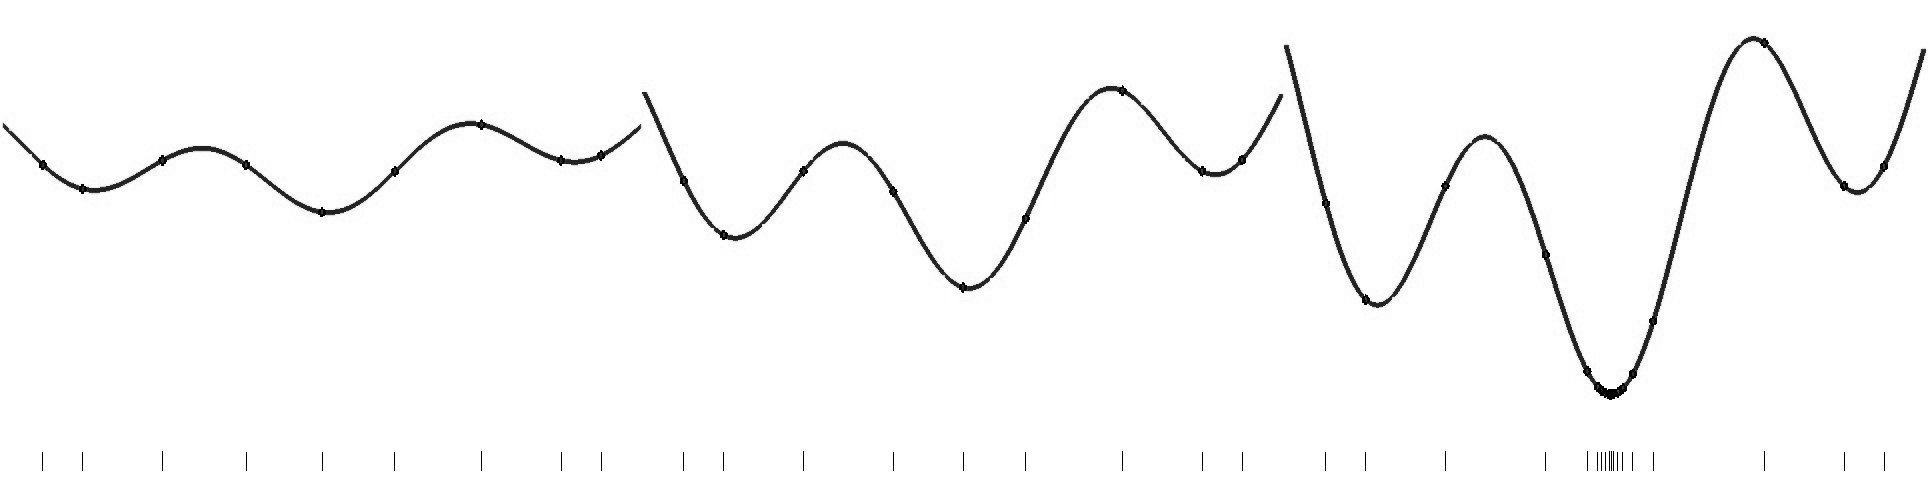
\includegraphics[width=0.9\textwidth]{fig1.jpg}
    \caption{Mixed-integer global optimization problem}
    \label{fig:1}
\end{figure}

By applying a parallel index algorithm with local tuning to the solution of problem  (\ref{problem_is1}), we find a solution to the problem  (\ref{problem_i}). In this case, the main part of the trials will be carried out in the subproblem, the solution of which corresponds to the solution of the original problem (\ref{problem_i}). In the remaining subtasks, only an insignificant part of the trials will be carried out, since solutions of these subproblems are locally optimal. This is confirmed by Fig. \ref{fig:1}, where the dashed lines indicate the trial points performed during the solution of this problem.

Thus, we have formed the Parallel Mixed-integer Global search Algorithm with Local tuning (PMGAL), based on the reduction of the mixed-integer non-convex optimization problem to a simultaneously solved set of continuous problems.

The proposed scheme for solving mixed-integer global optimization problems is based on a parallel index method for solving continuous optimization problems and is not oriented to a specific computing device.  One of the key operations here is the parallel execution of several trials at different points of the search domain (see step 7 of the algorithm), which can be implemented both on the CPU (using OpenMP and / or MPI) and on the GPU (using CUDA). 
In this work, parallelization was done only on CPUs. The workload was distributed between the nodes in accordance with the multilevel scheme of parallel computation decomposition described in \cite{Strongin2018,Barkalov2020}.

\section{Results of experiments}

The first series of experiments was carried out using a sequential version of the algorithm without using local tuning in order to compare it with other similar methods.
The PMGAL algorithm proposed in this work (in its sequential version) was compared with the genetic algorithm for solving mixed-integer optimization problems implemented in the Matlab Global Optimization Toolbox. Table \ref{tab:1} shows the number of trials and time it took for these methods to solve a number of mixed-integer test problems taken from \cite{Deep,Floudas}.  
%Russian
Использованные тестовые задачи содержали 2 непрерывных и 1 дискретный параметр, который имел от 3 до 6 значений в зависимости от задачи.
Также в постановку задач входили от 1 до 4 non-convex constraints. 
Отметим, что наличие сложных ограничений, которые формируют невыпуклую допустимую область, является препятствием к использованию методов, основанных на идеях локальной оптимизации. 
Генетический алгоритм из Matlab Global Optimization Toolbox использовался с рекомендованными параметрами (например, population size равнялся 50, максимальное число поколений -- 200, crossover fraction -- 0.8). The PMGAL algorithm использовался со стандартными параметрами, обеспечивающими сходимость к решению ( $r_\nu$ from (\ref{R}) равнялось 2.3 для всех $\nu = 1,2,3$, the evolvent construction parameter $M=10$).

The same accuracy of search $\epsilon = 10^{-2}$ was used for both methods.


All computational experiments were carried out on a computer with an Intel Core i5-7300 2.5 GHz processor and 8 Gb RAM. The experimental results show the superiority of the PMGAL method both in terms of the number of iterations and the running time.

\begin{table}[ht]
	\caption{Comparison of the effectiveness of the PMGAL and GA methods}
	\label{tab:1}
	\center
	\begin{tabular}{|c|c|c|c|c|}
		\hline
	\multirow{2}{*}{Test problem}	 & \multicolumn{2}{c|}{ GA } &  \multicolumn{2}{c|}{PMGAL} \\
		\cline{2-3} \cline{4-5} 
		 & Number of trials & Time, sec. &  Number of trials & Time, sec.  \\
		\hline 
		 Problem 2 \cite{Floudas}&	481 &	0.0601 & 	417 &	0.04 \\
		 Problem 6 \cite{Floudas}&	641 &	0.0510 & 	118 &	0.001 \\
		 Problem 1 \cite{Deep}   &	481 &	0.1378 & 	66 &	0.0007 \\
		 Problem 2 \cite{Deep}   &	481 &	0.0473 & 	57 &	0.0006 \\
		 Problem 7 \cite{Deep}   &	841 &	0.0736 &  372	 &	0.017 \\
		\hline
	\end{tabular}
\end{table}	


The next experiment was conducted to assess the effect of local tuning on accelerating the convergence of the algorithm. We used the GKLS generator \cite{Gaviano} to generate test problems of continuous multiextremal optimization. GKLS allows generating continuous functions of a given dimensionality with specific properties: a known number of local minima, a known domain of attraction of the global solution, etc.  
%This generator of multiextremal functions is often used for the investigations of the global optimization algorithms \cite{Paulavicius2014,SergeyevKvasov2015,Lebedev2015,Gergel2015}. 
Fig.~\ref{example} (a) and (b) shows the contour plots of two-dimensional GKLS functions. These figures also shows the points of the trials performed by the global search until the required accuracy $\epsilon=10^{-2}$ was achieved.

\begin{figure}[ht]
\begin{minipage}{0.48\linewidth}
\center{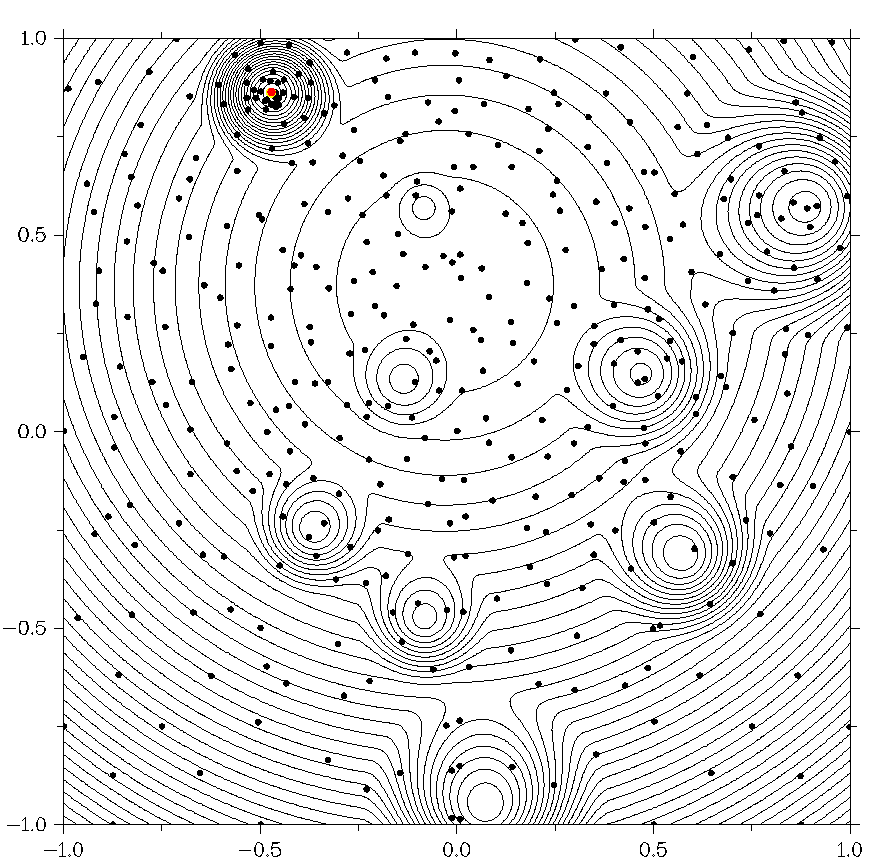
\includegraphics[width=1.0\linewidth]{GKLS-4.png} \\ (a)}
\end{minipage}
\hfill
\begin{minipage}{0.475\linewidth}
\center{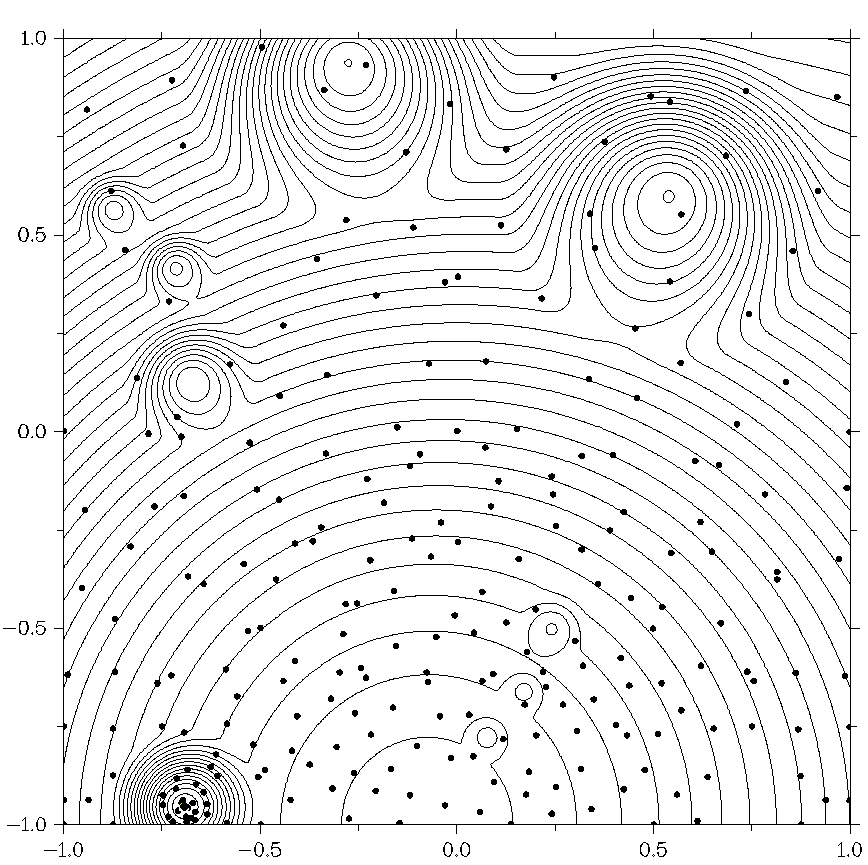
\includegraphics[width=1.0\linewidth]{GKLS-6.png} \\ (b)}
\end{minipage}
\caption{Solving a two-dimensional problem using the global search algorithm}
\label{example}
\end{figure}

In our experiments, the GKLS generator was used as a basis for constructing mixed-integer problems. The rules for generating trial problems of this type were as follows.

\begin{enumerate}
	\item GKLS generates a continuous multiextremal function $\psi(y), \; y\in D, \; D = \left\{ a_j\leq y_j\leq b_j, 1\leq j \leq N \right\}$. The global minimum of this function is achieved at the known point $y'=(y'_1,...,y'_N)$ and is equal to $\psi'=\psi(y')=-1$.
	\item A convex mixed-integer function
	\[
			\phi (y,u) = 2 \left[ \sum_{j=1}^N \left( \frac{y_j - y'_j}{b_j-a_j} \right)^2 + \sum_{j=1}^M \left( \frac{u_j - b_j}{b_j-a_j} \right)^2 \right]
	\]
	is generated, where 
	\begin{eqnarray*}
	& y\in D = \left\{ a_j\leq y_j\leq b_j, 1\leq j \leq N \right\} \subset R^N, \\
	& u\in U = \left\{ u_j \in  \left\{a_j, ..., b_j \right\}, 1\leq j \leq M \right\};
	\end{eqnarray*}
	i.e. this function has $N$ continuous and $M$ discrete parameters and reaches its minimum value at the point $(y',b)$.
	\item The coefficient
	\[
	C = 4 - \max \left\{ \phi(y,u) \right\}, \; y\in D, u \in U,
	\]
	is calculated. The maximum of the convex function $\phi(y,u)$ is achieved at one of the boundary points of the search domain; therefore, when the dimensionality of the problem is around 10, its calculation can be performed by the enumeration method. 
	\item  Multiextremal mixed-integer function
	\[
	\varphi(y,u) = \left(\psi(y) - \sum_{j=1}^M{u_j}\right)\left(C - \phi(y,u)\right)
	\]
	is formed. By construction, $\varphi(y,u)$ will reach the minimum value at the point $(y',b)$.
	
\end{enumerate}


The problems generated in our experiments had 5 discrete and 4 continuous parameters 
	\begin{eqnarray*}
	& y\in D = \left\{ -1 \leq y_j\leq 1, 1\leq j \leq 4 \right\} \subset R^4, \\
	& u\in U = \left\{ u_j \in  \left\{-1, -1/3, 1/3, 1 \right\}, 1\leq j \leq 5 \right\}.
	\end{eqnarray*}


In total, we generated and solved 100 mixed-integer problems of this type with 5 discrete and 4 continuous parameters. In order to simulate the computational complexity inherent in applied optimization problems, the calculation of the function in all the experiments was complicated by additional calculations that did not change the form of the function and the location of its minima.
The accuracy of the search was equal to $\epsilon = 10^{-2}$. Computational experiments were carried out on the Lobachevsky supercomputer. The node of supercomputer included two Intel Sandy Bridge E5-2660 2.2 GHz CPUs (16 cores in total) and 64 Gb RAM. 

Table \ref{tab:2} summarizes the experimental results obtained for the sequential version of the PMGAL algorithm using different strategies for alternating local and global search. For local search in formulas  (\ref{lR}), we used the parameter $q=3$, for global search -- $q=0$. The first column of the table shows the frequency of alternation of the indicated values. For example, 1:1 corresponds to alternating local and global search at each iteration; 1:2 corresponds to one local search step and two global search steps, and so on. The second column of the table reflects the average number of iterations  $K_{av}$ (thousand.), required to solve a problem with a given accuracy.

\begin{table}[ht]
	\caption{Comparison of local tuning strategies}
	\label{tab:2}
	\center
	\begin{tabular}{|c|c|}
		\hline		
		\textit{loc} : \textit{glob} & $K_{av}$   \\
		\hline 
		1 : 1 & 102.6\\
		1 : 2 & 89.2\\
		1 : 4 & 97.5\\
		1 : 8 & 127.1\\
		1 : 16 & 144.2\\
		\hline
	\end{tabular}
\end{table}	


Experimental results show that the least number of iterations is required for the method when using the 1:2 alternation strategy, i.e. one local refinement step alternates with two global search steps. We will use this strategy in further experiments.

%\begin{table}[ht]
	%\caption{Average running time $T_{av}$ of the parallel algorithm with local tuning}
	%\label{tab:3}
	%\center
	%\begin{tabular}{|c|c|c|c|}
		%\hline	
	%\diaghead{\theadfont Diag Column} { $N_{p}$}{$N_{t}$} & 1 & 4 & 8\\	
		%\hline		
		%2  & 199.0 & 65.4 & 61.0  \\
		%5  & 91.2 & 28.0 &  26.1 \\
		%17  & 37.2 & 10.8 & 7.5 \\
		%65  & 29.3 & 8.7 & 5.4 \\
		%\hline
	%\end{tabular}
%\end{table}	


The last experiment was performed to evaluate the acceleration of the parallel version of the PMGAL algorithm. 
%Russian
Параллельный алгоритм был применен с ранее использованными параметрами для решения той же серии из 100 problems with 5 discrete and 4 continuous parameters.
Fig.~ \ref{fig:3} shows the speedup $S(p)$ depending on the involved number of processes and threads in each process. Под ускореним здесь понимается отношение времени работы последовательного алгоритма $t_1$ ко времени работы параллельного $t_p$, т.е. $S(p) = t_1/t_p$, где $p$ -- суммарное число использованных threads.

Our experiments involved from 1 to 16 cluster nodes depending on the number of parallel processes. The speedup provided by the parallel algorithm is not ideal, but quite acceptable.

\begin{figure}[ht]
    \centering
    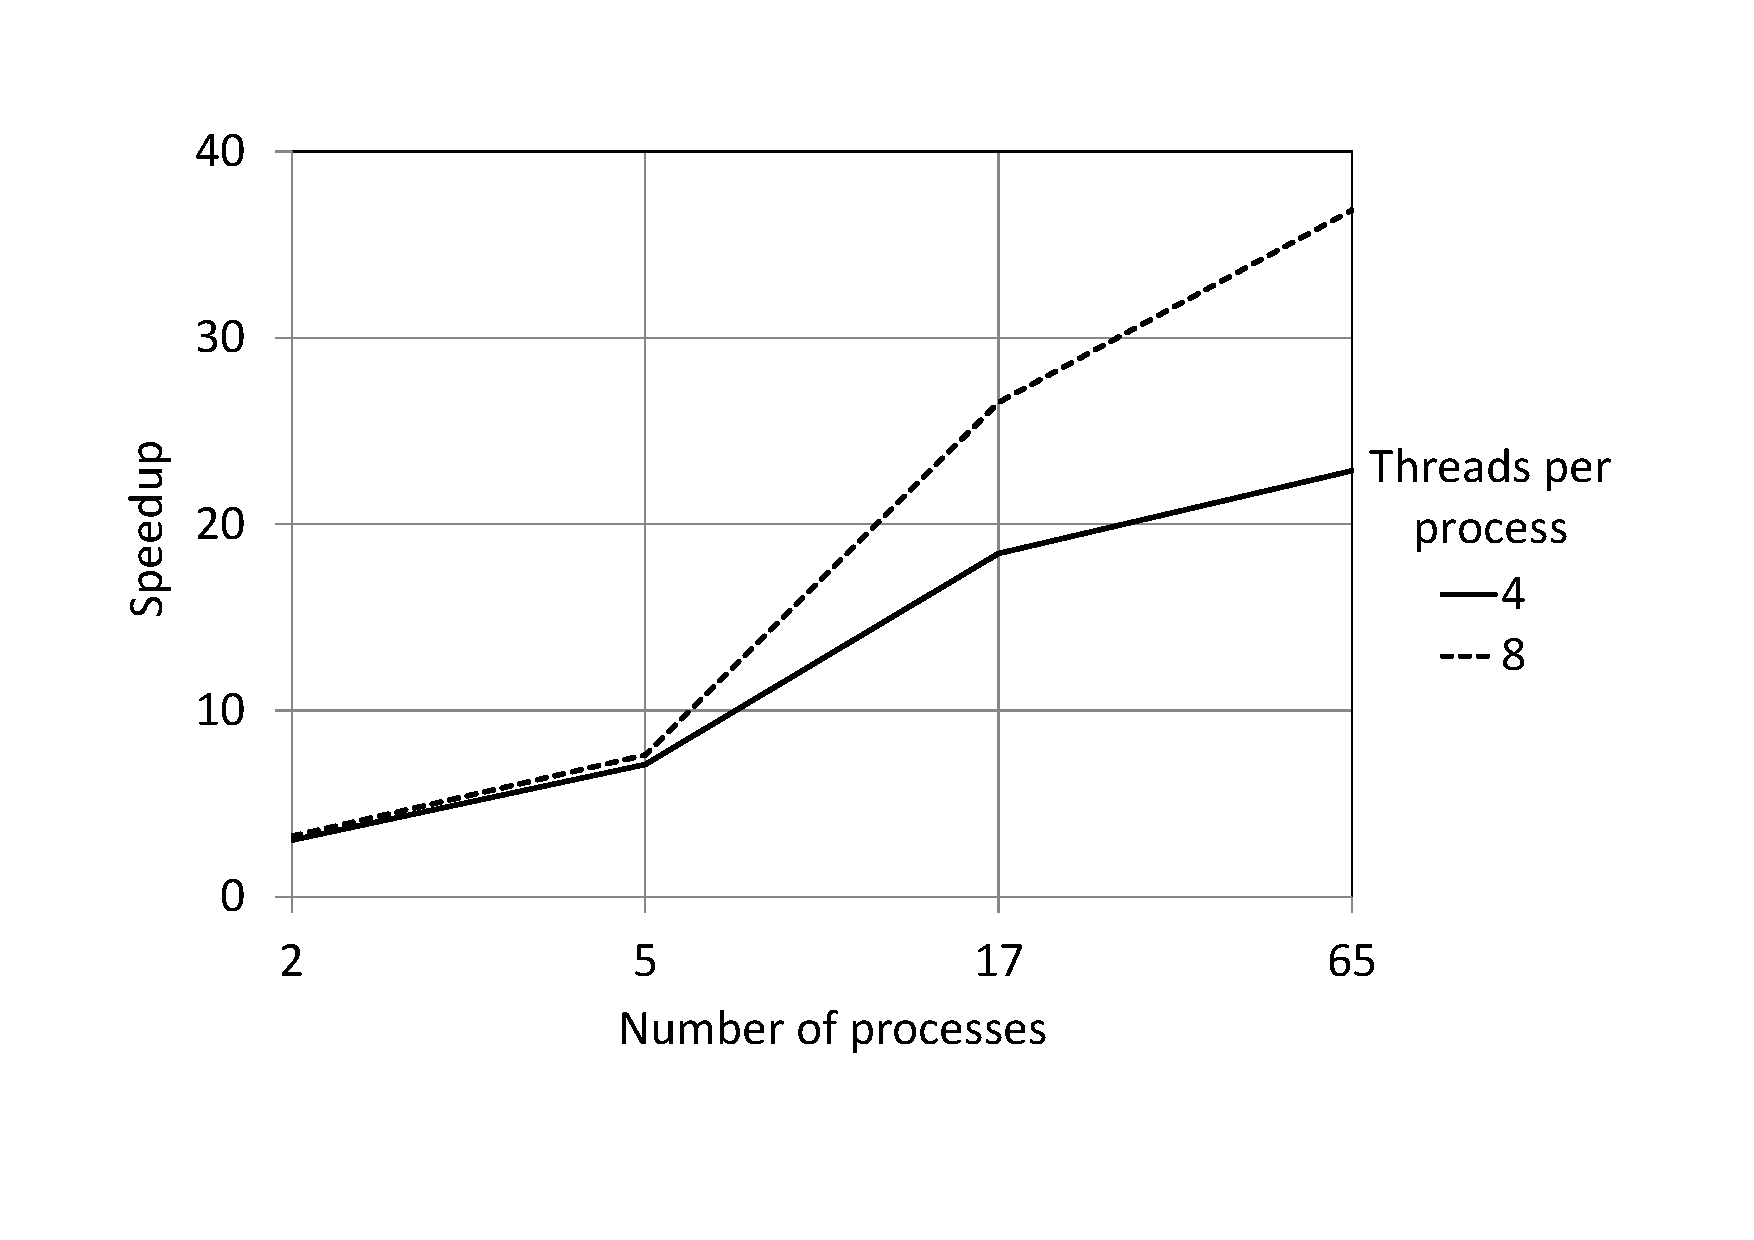
\includegraphics[width=0.6\textwidth]{speedup.pdf}
    \caption{Speedup of the parallel algorithm with local tuning}
    \label{fig:3}
\end{figure}




\section{Conclusions}

This article presents the results related to the development of parallel algorithms for global optimization for solving multiextremal problems in which some of the parameters are continuous, and some are discrete. 
These problems can also include non-convex constraints, which are accounted for using a special index scheme.

We propose a parallel algorithm for solving the problems of this class. The basic principle of organizing parallel computations in the algorithm is based on the simultaneous carrying out of several trials at different points of the search domain.
The parallel global optimization algorithm uses a local tuning technique based on the assumption that the multiextremity of the problem is weak. This assumption is true, in particular, at the final phase of the search, when one or more trials have already been performed in the vicinity of the global solution, and the only remaining step is to refine the found estimate of the solution.
In its sequential form, the proposed algorithm remains on par with the similar methods implemented in Matlab Global Optimization Toolbox. 
In a parallel form, the proposed algorithm demonstrates acceptable scalability up to dozens of parallel processes.

%Russian
Основным предположением, которое обеспечивает применимость предложенного алгоритма, является выполнение условия Липшица для функций задачи при варьировании непрерывных параметров для каждого фиксированного набора дискретных параметров.
Задачи оптимизации, в которых функции являются липшицевыми, относятся к классу вычислительно-трудоемких задач. Любой численный алгоритм решения такой задачи требует вычисления значений функции в узлах некоторой (равномерной или неравномерной) сетки во всей области допустимых изменений параметров.
Несмотря на то, что предположение липшицевости позволяет провести оценку оптимума на существенно неравномерной (т.е. более экономной по сравнению с равномерной) сетке в области поиска, масштаб решаемых задач здесь ограничен по сравнению с задачами на локальный экстремум. За приемлемое время даже с использованием параллельных алгоритмов можно решать задачи, в которых порядка 10 непрерывных и 10 дискретных параметров. 
Решение задач с сотнями переменных может быть основано на схеме вложенной оптимизации в предположении, что зависимость целевой функции от части переменных носит локальный характер \cite{Barkalov2020_1}.

Примером сложной прикладной задачи, к которой планируется применить разработанные алгоритмы, является выбор оптимальных параметров конструкции aircraft hot-air anti-icing system для самолетов российского производства. В математической модели anti-icing system наряду с параметрами, изменяющимися непрерывно (например, диаметр трубки, подводящей теплый воздух от двигателя в крыло; диаметр выпускных отверстий на данной трубке; расстояние между отверстиями; и т.п.), есть и дискретные параметры (например, число рядов выпускных отверстий, которое из технических ограничений может быть равно 1, 2 или 3). Пример подобной постановки задачи см. в \cite{Habashi}. Использование предложенного в статье алгоритма позволит не проводить оптимизацию для каждого значения дискретного параметра по отдельности, а заранее отсечь неперспективные варианты в процессе поиска. 
 


\begin{acknowledgments}
This work was supported by the Ministry of Science and Higher Education of the Russian Federation, project no. 0729-2020-0055, and by the Research and Education Mathematical Center, project no. 075-02-2020-1483/1.
\end{acknowledgments}


%
% The Bibliography
%

\begin{thebibliography}{99}

\bibitem{Burer}
S.~Burer and A.~N.~Letchford, \textit{Non-convex mixed-integer nonlinear programming: A survey}, Surveys in Operations Research and Management Science \textbf{17}, 97--106 (2012).

\bibitem{Boukouvala}
F.~Boukouvala, R.~Misener and C.~A.~Floudas, \textit{Global optimization advances in Mixed-Integer Nonlinear Programming, MINLP, and Constrained Derivative-Free Optimization, CDFO}, European J. Oper. Res. \textbf{252}, 701--727 (2016).

\bibitem{Belotti}
P.~Belotti, J.~Lee, L.~Liberti, F.~Margot and A.~W\"achter, \textit{Branching and bounds tightening techniques for non-convex MINLP}, Optim. Method. Softw. \textbf{24}(4-5), 597--634 (2009).

\bibitem{Vigerske}
S.~Vigerske and A.~Gleixner, \textit{SCIP: global optimization of mixed-integer nonlinear programs in a branch-and-cut framework}, Optim. Method. Softw. \textbf{33}(3), 563--593 (2018).

\bibitem{Deep}
K.~Deep, K.~P.~Singh, M.~L.~Kansal and C.~Mohan, \textit{A real coded genetic algorithm for solving integer and mixed integer optimization problems}, Appl. Math. Comput. \textbf{212}(2), 505--518 (2009).

\bibitem{Schluter}
M.~Schl\"uter, J.~A.~Egea and J.~R.~Banga, \textit{Extended ant colony optimization for non-convex mixed integer nonlinear programming}, Computers and Operations Research \textbf{36}(7), 2217--2229 (2009).

\bibitem{Strongin2000}
R.~G.~Strongin and Y.~D.~Sergeyev, \textit{Global optimization with non-convex constraints. Sequential and parallel algorithms} (Kluwer Academic Publishers, Dordrecht, 2000, 2nd ed. 2013, 3rd ed. 2014).

\bibitem{Strongin2013}
R.~G.~Strongin, V.~P.~Gergel, V.~A.~Grishagin and K.~A.~Barkalov, \textit{Parallel computations for global optimization problems} (Moscow State University, Moscow, 2013) [In Russian].

\bibitem{Evtushenko2009} 
Yu.~G.~Evtushenko, V.~U.~Malkova and A.~A.~Stanevichyus, \textit{Parallel global optimization of functions of several variables}, Computational Mathematics and Mathematical Physics \textbf{49}(2), 246--260 (2009).

\bibitem{Zilinskas2011}
R.~Paulavi\v{c}ius, J.~\v{Z}ilinskas and A.~Grothey, \textit{Parallel branch and bound for global optimization with combination of Lipschitz bounds}, Optimization Methods \& Software \textbf{26}(3), 487--498 (2011).

\bibitem{Zilinskas2014}
R.~Paulavi\v{c}ius and J.~\v{Z}ilinskas, \textit{Simplicial Global Optimization} (Springer Briefs in Optimization. Springer, 2014).

\bibitem{Sergeyev2017}
Y.~D.~Sergeyev and D.~E.~Kvasov, \textit{Deterministic Global Optimization. An Introduction to the Diagonal Approach}  (Springer Briefs in Optimization, Springer, 2017).


%\bibitem{Evtushenko2013} Y.~G.~Evtushenko and M.~A.~Posypkin, \textit{A deterministic approach to global box-constrained optimization}, Optim. Lett. \textbf{7}(4), 819--829 (2013).
	

\bibitem{Sergeyev2013}
Ya.~D.~Sergeyev, R.~G.~Strongin and D.~Lera, \textit{Introduction to Global Optimization Exploiting Space-Filling Curves} (Springer Briefs in Optimization, Springer, 2013).


\bibitem{Strongin2020}
R.~Strongin, K.~Barkalov and S.~Bevzuk, \textit{Global optimization method with dual Lipschitz constant estimates for problems with non-convex constraints}, Soft Computing \textbf{24}(16), 11853--11865 (2020).

\bibitem{Gergel2020}
V.~Gergel, E.~Kozinov and K.~ Barkalov, \textit{Computationally efficient approach for solving lexicographic multicriteria optimization problems}, Optim. Lett. (2020). DOI: 10.1007/s11590-020-01668-y 

\bibitem{Sergeyev2003}
Y.~D.~Sergeyev, P.~Pugliese and D.~Famularo, \textit{Index information algorithm with local tuning for solving multidimensional global optimization problems with multiextremal constraints}, Math. Program. \textbf{96}(3), 489--512 (2003).
2003.

\bibitem{Sergeyev2007}
Y.~D.~Sergeyev, D.~E.~Kvasov and F.~M.~H.~Khalaf, \textit{A one-dimensional local tuning algorithm for solving GO problems with partially defined constraints} Optimization Letters \textbf{1}(1), 85--99 (2007).

\bibitem{Sergeyev2020}
D.~E.~Kvasov, M.~S.~Mukhametzhanov, M.~C.~Nasso and Y.~D.~Sergeyev, \textit{On acceleration of derivative-free univariate Lipschitz global optimization methods}, Lecture Notes in Computer Science \textbf{11974}, 413--421 (2020).

\bibitem{Barkalov2010}
K.~Barkalov, V.~Ryabov, S.~Sidorov, \textit{Parallel scalable algorithms with mixed local-global strategy for global optimization problems}, Lecture Notes in Computer Science \textbf{6083}, 232–240 (2010).
 
\bibitem{Strongin2018}
R.~G.~Strongin, V.~P.~Gergel, K.~A.~Barkalov and A.~V.~Sysoyev, \textit{Generalized parallel computational schemes for time-consuming global optimization}, Lobachevskii Journal of Mathematics \textbf{39}(4), 576--586 (2018.)

\bibitem{Barkalov2020}
R.~G.~Strongin, V.~P.~Gergel and K.~A.~Barkalov, \textit{Adaptive global optimization based on a block-recursive dimensionality reduction scheme}, Automation and Remote Control \textbf{81}(8), 1475--1485 (2020).

\bibitem{Floudas}
C.~A.~Floudas and M.~P.~Pardalos,  \textit{Handbook of Test Problems in Local and Global Optimization}. (Springer, 1999).  %; DOI: 10.1007/978-1-4757-3040-1

\bibitem{Gaviano}
M.~Gaviano, D.~Lera, D.~E.~Kvasov and Y.~D.~Sergeyev, \textit{Software for generation of classes of test functions with known local and global minima for global optimization}, ACM Trans. Math. Softw. \textbf{29}, 469--480 (2003).

\bibitem{Barkalov2020_1}
K.~Barkalov, I.~Lebedev, M.~Kocheganova, V.~Gergel, \textit{Combining local and global search in a parallel nested optimization scheme}, Communications in Computer and Information Science, \textbf{1263}, 100-112 (2020).

\bibitem{Habashi}
M.~P.~C. Pellissier, W.~G. Habashi, A.~Pueyo. \textit{Optimization via FENSAP-ICE of aircraft hot-air anti-icing systems}, Journal of Aircraft \textbf{48}(1), 265--276 (2011). 





%\bibitem{Floudas}
%C.~A.~Floudas and M.~P.~Pardalos, \textit{Recent advances in global optimization} (Princeton University Press, 2016).
%
%\bibitem{Locatelli}
%M.~Locatelli and F.~Schoen, \textit{Global optimization: theory, algorithms and applications} (SIAM, 2013).
%
%
%\bibitem{Pardalos}
%P.~M.~Pardalos, A.~A.~Zhigljavsky and J.~\v{Z}ilinskas \textit{Advances in stochastic and deterministic global optimization} (Springer, 2016).
%
%
%\bibitem{Ciegis}
%R.~\v{C}iegis, D.~Henty, B.~K\r{a}gstr\"om and J.~\v{Z}ilinskas, \textit{Parallel scientific computing and optimization: advances and applications}  (Springer, 2009). 
%
%\bibitem{Luque}
%G.~Luque and E.~Alba, \textit{Parallel genetic algorithms. Theory and real world applications} (Springer-Verlag, Berlin, 2011).
%
%\bibitem{Strongin3}
%R.~G.~Strongin, \textit{Numerical Methods in Multiextremal Problems (Information-Statistical Algorithms)} (Nauka, Moscow, 1978) [In Russian].
%
%\bibitem{Strongin4}
%R.~G.~Strongin and Y.~D.~Sergeyev, \textit{Global multidimensional optimization on parallel computer}, Parallel Computing \textbf{18} (11), 1259--1273 (1992).
%
%\bibitem{Sergeyev4}
%Y.~D.~Sergeyev and V.~A.~Grishagin, \textit{Parallel asynchronous global search and the nested optimization scheme}, J. Comput. Anal. Appl., \textbf{3} (2), 123--145 (2001).
%
%\bibitem{Gergel1}
%V.~P.~Gergel and S.~V.~Sidorov, \textit{A Two-Level Parallel Global Search Algorithm for Solution of Computationally Intensive Multiextremal Optimization Problems}, Lecture Notes in Computer Science \textbf{9251}, 505--515 (2015).
%
%\bibitem{Gergel2}
%V.~Gergel, \textit{An Unified Approach to Use of Coprocessors of Various Types for Solving Global Optimization Problems}, in Proceedings of the Second International Conference on Mathematics and Computers in Sciences and in Industry (MCSI), Sliema, 13--18 (2015).
%
%\bibitem{Barkalov}
%K.~Barkalov, V.~Gergel and I.~Lebedev, \textit{Solving global optimization problems on GPU cluster}, AIP Conference Proceedings \textbf{1738}, 400006 (2016).
%
%\bibitem{Gergel3}
%V.~Gergel and E.~Kozinov, \textit{Efficient methods of multicriterial optimization based on the intensive use of search information}, Springer Proceedings in Mathematics and Statistics \textbf{197}, 27--45 (2017). 
%
%\bibitem{Gergel4}
%V.~Gergel and E.~Kozinov, \textit{Parallel computing for time-consuming multicriterial optimization problems}, Lecture Notes in Computer Science \textbf{10421}, 446--458 (2017).
%
%\bibitem{Gergel5}
%V.~Gergel, V.~Grishagin and A.~Gergel, \textit{Adaptive nested optimization scheme for multidimensional global search}, J. Glob. Optim.  \textbf{66} (1), 35--51 (2016).
%
%\bibitem{Lera}
%D.~Lera, Y.~D.~Sergeyev, \textit{Lipschitz and Holder global optimization using space-filling curves},  Appl. Numer. Math. \textbf{60} (1-2), 115--129 (2010).
%
%\bibitem{Grishagin1}
%V~A.~Grishagin. \textit{On convergence conditions for a class of global search algorithms}, in Proceedings of the 3-rd All-Union seminar ``Numerical methods of nonlinear programming'', Kharkov, 82--84 (1979) [In Russian].
%
%\bibitem{Grishagin2}
%V.~A.~Grishagin, Y.~D.~Sergeyev and R.~G.~Strongin, \textit{Parallel characteristic algorithms for solving problems of global optimization}, J. Glob. Optim. \textbf{10} (2), 185--206 (1997).
%
%\bibitem{Strongin5}
%R.~G.~Strongin, \textit{Algorithms for Multi-extremal Mathematical Programming Problems Employing the Set of Joint Space-filling Curves}, J. Glob. Optim. \textbf{2} (4), 357--378 (1992).
%
%\bibitem{Sysoyev}
%A.~Sysoyev, K.~Barkalov, V.~Sovrasov, I.~Lebedev and V.~Gergel, \textit{Globalizer -- A parallel software system for solving global optimization problems}, Lecture Notes in Computer Science \textbf{10421}, 492--499 (2017). 
%
%\bibitem{Sergeyev7}
%Y.~D.~Sergeyev and V.~A.~Grishagin, \textit{Parallel Asynchronous Global Search and the Nested Optimization Scheme}, J. Comput. Anal. Appl. \textbf{3} (2), 123--145 (2001).
%
%\bibitem{Modorskii}
%V.~Y.~Modorskii, D.~F.~Gaynutdinova, V.~P.~Gergel and K.~A.~Barkalov, \textit{Optimization in design of scientific products for purposes of cavitation problems}, AIP Conference Proceedings \textbf{1738}, 400013 (2016).
%
%\bibitem{Gergel6}
%V.~P.~Gergel, M.~I.~Kuzmin, N.~A.~Solovyov and V.~A.~Grishagin, \textit{Recognition of surface defects of cold-rolling sheets based on method of localities}, International Review of Automatic Control \textbf{8} (1), 51--55 (2015).


\end{thebibliography}
\end{document}
